%%%%%%%%%%%%%%%%%%%%%%%%%%%%%%%%%%%%%%%%%%%%%%%%%%%%%%%%
%%
\clearpage
\newpage
\section{The cal\_ recipe}
\label{ch:the_recipes:cal_}
%%
%%%%%%%%%%%%%%%%%%%%%%%%%%%%%%%%%%%%%%%%%%%%%%%%%%%%%%%%



% % -------------------------------------------------------
% \subsection{The inputs}
% % -------------------------------------------------------
% The input of \_ is as follows:
% \begin{cmdbox}

% \end{cmdbox}
% \noindent for example
% \begin{cmdbox}[title={example}]

% \end{cmdbox}
% \noindent or
% \begin{pythonbox}
% import 

% cal_DARK_spirou.main()
% \end{pythonbox}

% \noindent where `night\_repository' defines \argnightname and `filenames' define the list of files in \argfilenames. All files in filenames must be valid python strings separated by a space (command line) or in a line (python) and must have the folowing prefixes:
% \begin{itemize}
% 	\item {}
% \end{itemize}

% % -------------------------------------------------------
% \subsection{The outputs}
% % -------------------------------------------------------
% The outputs of \_ are as follows:

% \begin{itemize}

% \item \definevariable{}{} in form:
% \begin{tcustomdir}
% \{\reduceddir\}/\{date prefix\}\_\{file\}.fits
% \end{tcustomdir}

% \end{itemize}


% \noindent where `date prefix' is constructed from \argnightname and the file name is the first file in \argfilenames.


% \noindent for example for \reduceddir\lstinline[style=pythoninline]|='/drs/data/reduced/20170710'| and \argfilenames\lstinline[style=pythoninline]|=['']| the output files would be:
% \begin{tcustomdir}
% \begin{itemize}
% \item \path{/drs/data/reduced/20170710/20170710\_ }
% \item \path{/drs/data/reduced/20170710/20170710\_ }
% \end{itemize}
% \end{tcustomdir}

% % -------------------------------------------------------
% \subsection{Summary of procedure}
% % -------------------------------------------------------
% \begin{enumerate}
% \item {}
% \end{enumerate}


% % -------------------------------------------------------
% \subsection{Quality Control}
% % -------------------------------------------------------

% Text here
% \begin{itemize}
% \item condition here
% \begin{thighlight}
% \begin{equation}
% Equation
% \end{equation}
% \end{thighlight}

% \end{itemize}

% \noindent If none of these quality control criteria are valid then the output file is passed into the \calibdb with key `KEY' for the `'. \\

% \noindent For example the following lines are added to the \calibdb for 
% \argnightname{\lstinline[style=pythoninline]| = "20170710" |} and \argfilenames{\lstinline[style=pythoninline]| = "" |}. \\

% \begin{textbox}[title={In calibration database file}]

% \end{textbox}


% % -------------------------------------------------------
% \newpage
% \subsection{Example working run}
% % -------------------------------------------------------

% An example run where everything worked is below:

% \begin{cmdboxprintspecial}[fontupper=\tiny, fontlower=\tiny]
% @g

% @g
% \end{cmdboxprintspecial}


% % -------------------------------------------------------
% \newpage
% \subsection{Interactive mode}
% % -------------------------------------------------------

% \noindent In interactive mode three figures will also appear (see Figure \ref{figure:}).

% \begin{figure}

% \begin{center}
% \begin{minipage}{.495\textwidth}
% \begin{center}
% \includegraphics[width=\textwidth]{Figures/cal_DARK_spirou_1.pdf}
% a
% \end{center}
% \end{minipage}%
% \begin{minipage}{.495\textwidth}
% \begin{center}
% \includegraphics[width=\textwidth]{Figures/cal_DARK_spirou_2.pdf}
% b
% \end{center}
% \end{minipage}%
% \end{center}

% \begin{center}
% \begin{minipage}{.495\textwidth}
% \begin{center}
% \includegraphics[width=\textwidth]{Figures/cal_DARK_spirou_3.pdf}
% c
% \end{center}
% \end{minipage}%
% \end{center}

% \caption{\textbf{(a)} The image with overplot red and blue regions (red/blue rectangles). \textbf{(b)} The bad pixel mask, bad pixels have a value=1 (in black) and good pixels have a value=0 (in white). \textbf{(c)} Histograms of the image regions, the full image (in green), the blue section (in blue) and the red section (in red). \label{figure:cal_DARK_spirou}}
% \end{figure}